\chapter{Browser testing}
The TS interface officially supports the latest ESR release of Mozilla Firefox.
However, user tend to use many different browsers. When developing new interfaces
it is very unpractical to test all these browsers manually and consistently.

Also, because of the frequent changes made to web browsers (described in chapter \ref{Evergreen browsers}),
it has become very important to test interface functionality as browser versions
get updated at production systems.

\section{Selenium}
Selenium is a tool that can automate a browser. Its most common uses are to
perform tests or to automate web interfaces.

Starting from version 2, it uses an open standard called `WebDriver` to interact
with a browser. Most modern browsers have a native implementation of this standard,
and separate drivers exist for browsers that do not (including IE6).

Selenium can run under Windows, Mac OS X, and Linux (Debian \& RHEL).
It has official libraries for C#, Haskell, Java, JavaScript (Node.js), Objective-C,
Perl, PHP, Python, R, and Ruby.

\section{Web-component-tester}
The polymer project contains a dedicated testing tool to test Polymer elements and
is used in the TS.

It allows a developer to make a series of tests for every Polymer element (and thus
every interface). These tests are performed using the grunt build system when
executing `grunt test`.

Tests are defined in a `test` folder in the source folder of every element.
There a developer can define tests with the `test()` function like this:

\fvset{frame=single}
\begin{pyglist}[language=javascript,numbers=left,numbersep=5pt,fontsize=\small]
// this function tests if the Polymer element has declared an object
// `someObject` and it has a property `name` with value `deinonychus`
test('defines the "author" property', function() {
    assert.equal(element.someObject.name, 'deinonychus');
});
// tests if the function `sayHello()` returns a specific string.
// also tests if the function `sayHello()` respects its arguments.
test('says hello', function() {
    assert.equal(element.sayHello(), 'template-element says, Hello World!');
    var greetings = element.sayHello('greetings Earthlings');
    assert.equal(greetings, 'template-element says, greetings Earthlings');
});
\end{pyglist}
\fvset{frame=none}

More advanced use cases, such as testing AJAX (Asynchronous JavaScript And XML) requests
or even emulating an AJAX response are also possible.
More detailed examples of web-component-tester can be found in the Sphinx documentation,
which can be found in appendix \ref{appendix_sphinx}.

When a developer executes `grunt test`, a Selenium server is started and the
defined tests are performed using the latest version of Mozilla~Firefox,
Google~Chrome, Google~Chrome~Canary, and Safari (if possible).

\begin{figure}
  \centering
  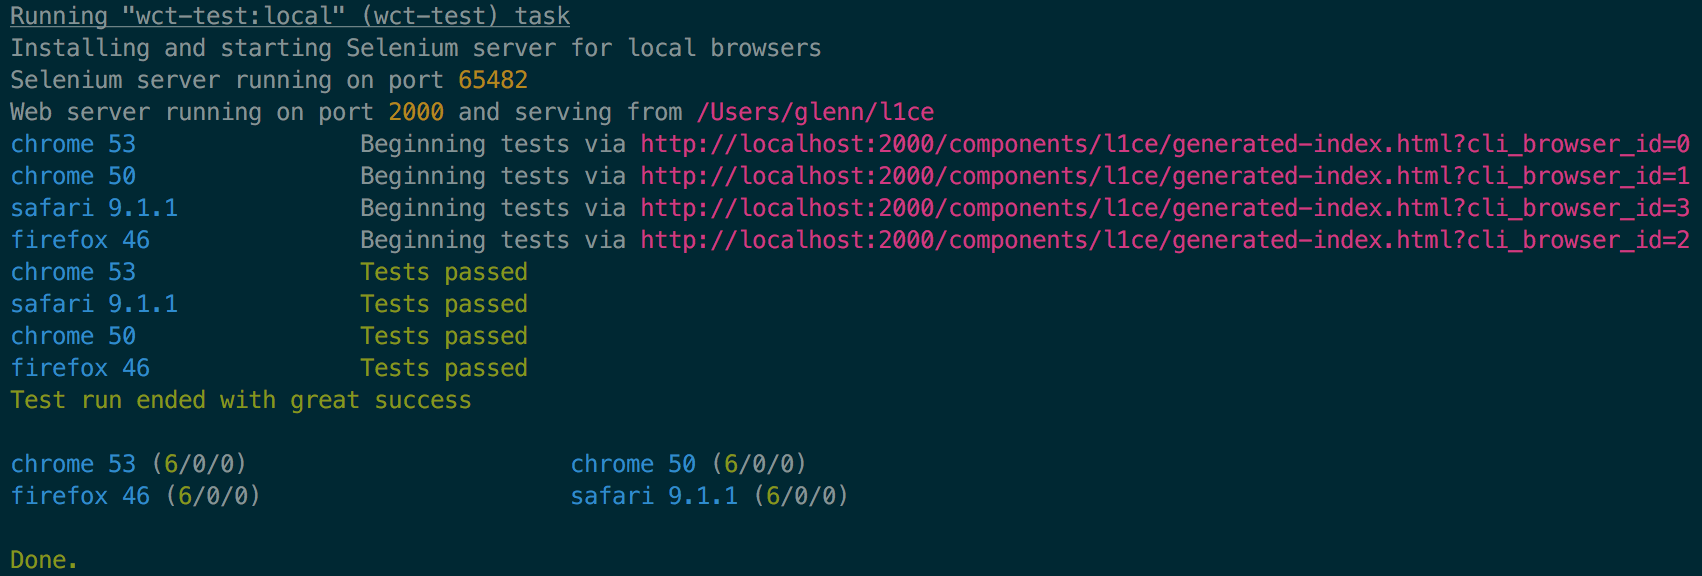
\includegraphics[width=\textwidth]{images/grunt_test}
  \caption{Console output when running tests with web-component-tester}
  \label{fig:grunt_test}
\end{figure}
